
%(BEGIN_QUESTION)
% Copyright 2010, Tony R. Kuphaldt, released under the Creative Commons Attribution License (v 1.0)
% This means you may do almost anything with this work of mine, so long as you give me proper credit

Beregn nedre og øvre måleverdi for denne nivåtransmitteren ut fra informasjonen i diagrammet nedenfor. Anta at transmitterens ``lav''-side er ventilert til atmosfæren. Oppgi svarene i enheten tommer vannsøyle ("W.C.):

$$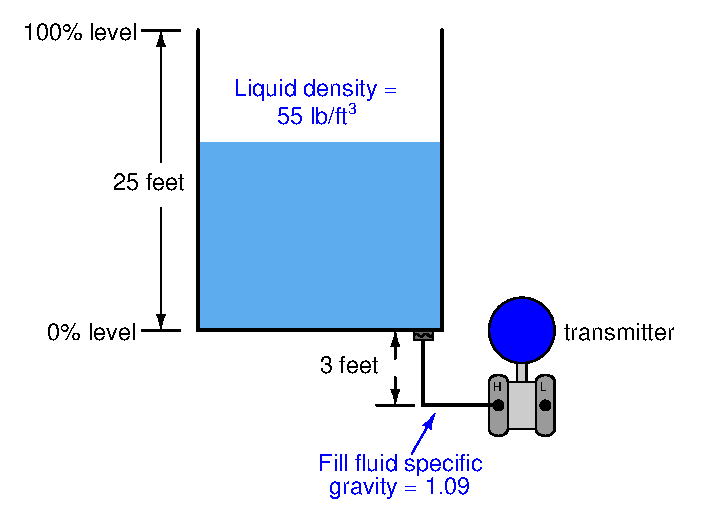
\includegraphics[width=15.5cm]{i00504x01.eps}$$

LRV = \underbar{\hskip 50pt} "W.C. \hskip 100pt URV = \underbar{\hskip 50pt} "W.C.

\underbar{file i00504}
%(END_QUESTION)





%(BEGIN_ANSWER)

LRV = \underbar{\bf 39.24} "W.C. \hskip 100pt URV = \underbar{\bf 303.7} "W.C.

%(END_ANSWER)





%(BEGIN_NOTES)

{\bf Denne oppgaven er ment for eksamen, ikke arbeidsark!}.

%(END_NOTES)

